\documentclass[oneside,letterpaper,12pt]{book}
\usepackage[T1]{fontenc}
\usepackage[top=0.8874in,bottom=0.8874in,left=0.7874in,right=0.7874in]{geometry}
\usepackage{charter}
\usepackage{lmodern}
\usepackage{amssymb,amsmath}
\usepackage{ifxetex,ifluatex}
\usepackage{fixltx2e} % provides \textsubscript
\ifnum 0\ifxetex 1\fi\ifluatex 1\fi=0 % if pdftex
  \usepackage[T1]{fontenc}
  \usepackage[utf8]{inputenc}
\else % if luatex or xelatex
  \ifxetex
    \usepackage{mathspec}
  \else
    \usepackage{fontspec}
  \fi
  \defaultfontfeatures{Ligatures=TeX,Scale=MatchLowercase}
\fi
% use upquote if available, for straight quotes in verbatim environments
\IfFileExists{upquote.sty}{\usepackage{upquote}}{}
% use microtype if available
\IfFileExists{microtype.sty}{%
\usepackage[]{microtype}
\UseMicrotypeSet[protrusion]{basicmath} % disable protrusion for tt fonts
}{}
\PassOptionsToPackage{hyphens}{url} % url is loaded by hyperref
\usepackage[unicode=true]{hyperref}
\hypersetup{
            pdfauthor={Gregory Raven},
            pdfborder={0 0 0},
            breaklinks=true}
\urlstyle{same}  % don't use monospace font for urls
\usepackage{graphicx,grffile}
\makeatletter
\def\maxwidth{\ifdim\Gin@nat@width>\linewidth\linewidth\else\Gin@nat@width\fi}
\def\maxheight{\ifdim\Gin@nat@height>\textheight\textheight\else\Gin@nat@height\fi}
\makeatother
% Scale images if necessary, so that they will not overflow the page
% margins by default, and it is still possible to overwrite the defaults
% using explicit options in \includegraphics[width, height, ...]{}
\setkeys{Gin}{width=\maxwidth,height=\maxheight,keepaspectratio}
\IfFileExists{parskip.sty}{%
\usepackage{parskip}
}{% else
\setlength{\parindent}{0pt}
\setlength{\parskip}{6pt plus 2pt minus 1pt}
}
\setlength{\emergencystretch}{3em}  % prevent overfull lines
\providecommand{\tightlist}{%
  \setlength{\itemsep}{0pt}\setlength{\parskip}{0pt}}
\setcounter{secnumdepth}{0}
% Redefines (sub)paragraphs to behave more like sections
\ifx\paragraph\undefined\else
\let\oldparagraph\paragraph
\renewcommand{\paragraph}[1]{\oldparagraph{#1}\mbox{}}
\fi
\ifx\subparagraph\undefined\else
\let\oldsubparagraph\subparagraph
\renewcommand{\subparagraph}[1]{\oldsubparagraph{#1}\mbox{}}
\fi

% set default figure placement to htbp
\makeatletter
\def\fps@figure{htbp}
\makeatother


\title{Mongoose-OS ESP32 Temperature Sense with Websocket and D3.js Display}
\author{Gregory Raven}
\date{October 28, 2017}

\begin{document}
\maketitle

{
\setcounter{tocdepth}{2}
\tableofcontents
}
\chapter{Introduction}\label{introduction}

This is the documentation for a project based on the Mongoose-OS
operating system. The development board contains an ESP32
system-on-chip. A DHT22 temperature-humidity sensor chip is wired to the
ESP32 board.

The system is an HTTP5 web server. The server provides a web page which
then connects to the server via Websocket. The browser must be Websocket
capable. After a Websocket connection is established, the server begins
publishing JSON data. The data is received by the web page via embedded
Javascript code. D3.js visualization is used to plot the incoming
temperature data versus time. An example plot is shown below.

\begin{figure}
\centering
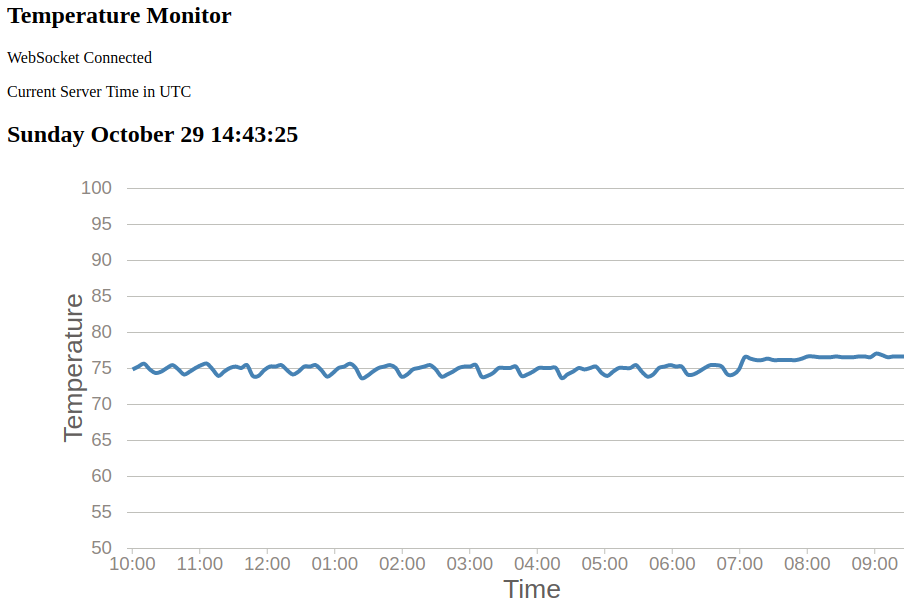
\includegraphics{tempviz1.png}
\caption{D3.js Plot of Temperature Data from the ESP32}
\end{figure}

A note of caution on this project. None of the available security
features are enabled. This project should only be deployed in a local
network behind a firewall. It should not be ``internet facing''.

Assembly of the project can be done on an inexpensive breadboard. Most
of the ESP32 development boards should work, however, some of them have
wide pin-spacings which do not work well with the common breadboard. The
latest board from Adafruit, the ``Feather'' board is the narrowest seen
yet, allowing two rows of pins on one side and one side on the other.
This board also had capability for battery power which is a nice
feature.

(insert Adafruit board/project image here)

\chapter{Mongoose-OS Code on the
ESP32}\label{mongoose-os-code-on-the-esp32}

This chapter describes the Mongoose-OS code used with the ESP32.

The code is all done in C. A Javascript version may be published in the
future. C was chosen as the author was interested in learning embedded C
programming. There is substantial Javascript code in the web page which
receives and displays data.

Using the built-in capability of Mongoose-OS, the code is surprisingly
simple. The libraries and facilities provided make the web server code
brief; perhaps even simpler than using a high-level framework like
Node.js.

\section{\texorpdfstring{Creating an ``Empty
App''}{Creating an Empty App}}\label{creating-an-empty-app}

Install the mos tool per the instructions:

\url{https://mongoose-os.com/software.html}

The author prefers operating at the command line in Linux. However,
everything described should be possible using the mos GUI, which is
launched as follows:

\begin{verbatim}
mos ui
\end{verbatim}

Create the ``empty app'' as follows:

\begin{verbatim}
mkdir websocket_send_periodic_temp
cd websocket_send_periodic_temp
mos init --arch=esp32
\end{verbatim}

The above command will create the file structure necessary to build the
app with the mos tool.

\section{\texorpdfstring{``Main''
Function}{Main Function}}\label{main-function}

It is not ``main'' as in typical C programming. For Mongoose-OS, the
entry function is called ``mgos\_app\_init(void)''.

\begin{verbatim}
enum mgos_app_init_result mgos_app_init(void) {
    struct mg_connection * nc;
    void * user_data = "";
    bool dhtInit;

    //  1. Get the server handle.
    if((nc = mgos_get_sys_http_server()) == NULL) {
        puts("The value of nc is NULL");
    }

    //  2. Bind the event handler to the HTTP server.
    mgos_register_http_endpoint("/", ev_handler, user_data);

    //  3. Create the DHT22 sensor.
    if((dht11 = mgos_dht_create(2, DHT22)) == NULL) {
        puts("DHT22 handle not created");
    }

    //  4.  Initialize the sensor.
    dhtInit = mgos_dht_init();
    if(dhtInit) {
        puts("DHT sensor initialized.");
    }

    return MGOS_APP_INIT_SUCCESS;
}
\end{verbatim}

The four significant lines above get the http server and the sensor
primed for operation:

\begin{enumerate}
\def\labelenumi{\arabic{enumi}.}
\tightlist
\item
  mgos\_get\_sys\_http\_server() is the entire invocation of a
  Mongoose-OS http server!
\item
  Since the system will be responsive to events, an event handler
  function ``ev\_handler'' is bound to the http server.
\item
  The DHT22 sensor object is created. Note that a DHT22 device is used,
  as it has better resolution than the DHT11.
\item
  The last step is to initialize the sensor.
\end{enumerate}

That is all, it is very easy!

\section{Configuration}\label{configuration}

Note that the ``empty app'' does not include the http server and DHT22
device related code. Mongoose-OS partitions these features into
``libraries'' which must be incorporated into the app. There are two
steps which are required to activate these features:

\begin{enumerate}
\def\labelenumi{\arabic{enumi}.}
\tightlist
\item
  Add the libraries to the mos.yml file. A default mos.yml file is
  created by the mos init command. Add the http-server and dht lines to
  the mos.yml file. The ``libs'' section of the file should look like
  this:
\end{enumerate}

\begin{verbatim}
# List of libraries used by this app, in order of initialisation
libs:
  - origin: https://github.com/mongoose-os-libs/ca-bundle
  - origin: https://github.com/mongoose-os-libs/rpc-service-config
  - origin: https://github.com/mongoose-os-libs/rpc-service-fs
  - origin: https://github.com/mongoose-os-libs/rpc-uart
  - origin: https://github.com/mongoose-os-libs/wifi
  - origin: https://github.com/mongoose-os-libs/http-server
  - origin: https://github.com/mongoose-os-libs/dht
\end{verbatim}

The libraries are described here:

\url{https://mongoose-os.com/docs/reference/api.html}

\begin{enumerate}
\def\labelenumi{\arabic{enumi}.}
\setcounter{enumi}{1}
\tightlist
\item
  Add the \#include lines to the main.c file. The top of the file should
  look like this:
\end{enumerate}

\begin{verbatim}
#include "mgos.h"
#include "mgos_http_server.h"
#include "mgos_dht.h"
\end{verbatim}

\section{The Event Handler Function}\label{the-event-handler-function}

The ``Event Handler'' function responds to events generated by the http
server. This includes Websocket events. The events are fired by
Mongoose-OS, and the event handler uses a switch statement to deal with
each individual type of event as required.

The events can be determined by examining the mongoose.h header file. It
is recommended to download the Mongoose-OS git repository and study the
header file:

\url{https://github.com/cesanta/mongoose-os}

The file is found in the directory mongoose.

Other examples of event handlers can be found in the example apps:

\url{https://mongoose-os.com/docs/reference/apps.html}

Here is the source code:

\begin{verbatim}
static void ev_handler(struct mg_connection *nc, int ev, void *ev_data, void *user_data) {
    struct http_message *hm = (struct http_message *) ev_data;
    switch (ev) {
    case MG_EV_HTTP_REQUEST: {             // #1 HTTP request
        mg_serve_http(nc, hm, http_opts);
        break;
    }
    case MG_EV_SEND: {
        // puts("MG_EV_SEND event fired!");
        break;
    }
    case MG_EV_WEBSOCKET_HANDSHAKE_DONE: {
        //  This sets the periodic time updating in motion.
        mg_set_timer(nc, mg_time() + INTERVAL_SECONDS);  // #2 Timer initialization.
        break;
    }
    case MG_EV_WEBSOCKET_FRAME: {
        // printf("Websocket message received:\n");
        break;
    }
    case MG_EV_CLOSE: {
        break;
    }
    //  The timer event causes a JSON string to be sent to the
    //  webpage via Websocket.
    case MG_EV_TIMER: {          //  #3 Most of the action is here!
        maintime = time(NULL);
        localstruct = localtime(&maintime);
        //  printf("The seconds are %d.\n", localstruct->tm_sec);
        strftime(utctime, sizeof(utctime), "%A %B %d %T", localstruct);
        tempC = mgos_dht_get_temp(dht11);
        //  printf("The temperature in degrees C is %2.1f.\n", ctof(tempC));
        humidity = mgos_dht_get_humidity(dht11);
        //  printf("The humidity in percent is %2.1f.\n", humidity);
        //  printf("Time is %s.\n", utctime);
        //  #4 Update time every 1 second; temp and humidity every five minutes.
        mg_printf_websocket_frame(nc, WEBSOCKET_OP_TEXT, timeString, utctime);
        if (count == 300) {
            mg_printf_websocket_frame(nc, WEBSOCKET_OP_TEXT, tempString, ctof(tempC));
            mg_printf_websocket_frame(nc, WEBSOCKET_OP_TEXT, humidString, humidity);
            count = 0;
        }
        count++;
        //  A new timer is set.
        mg_set_timer(nc, mg_time() + INTERVAL_SECONDS);
        break;
    }
    }
}
\end{verbatim}

The event handler function must follow the correct prototype pattern.
Again, refer to the header file mongoose.h.

Mongoose-OS takes care of calling the event handler function when it is
required. This is a fundamental feature of the OS and the http-server
library. All is built-in and nicely integrated with WIFI. WIFI
configuration will be covered later.

The developer is responsible for customizing the event handler to meet
the system's requirements. This is where the action happens with regards
to what behavior is desired from the system.

Note that several unused event types appear in the source code fragment.
These were left in place to show other possible Mongoose-OS events. Now
to describe the events used in this project:

\begin{enumerate}
\def\labelenumi{\arabic{enumi}.}
\tightlist
\item
  MG\_EV\_HTTP\_REQUEST. This is the usual response to an http ``get''
  request, and this sends the response. In terms of this project, this
  will be the html and embedded javascript, and the style sheet. The
  event handler is bound to the ``root'' which is ``/''. In use the URL
  will be as follows, making the assumption the IP address is
  192.168.1.4:
\end{enumerate}

\begin{verbatim}
     http://192.168.1.4/websocketweather.html
\end{verbatim}

\begin{enumerate}
\def\labelenumi{\arabic{enumi}.}
\setcounter{enumi}{1}
\tightlist
\item
  MG\_EV\_WEBSOCKET\_HANDSHAKE\_DONE. This event is fired upon
  completion of the Websocket handshake process. This sets the Mongoose
  timer in motion, and Websocket messages will begin to flow.
\item
  MG\_EV\_TIMER. This event is fired at the expiration of the Mongoose
  timer. This event creates all of the action in this project. The timer
  is initially set in step \#2, and then re-set in this branch of the
  switch statement. The function ``mg\_printf\_websocket\_frame'' is
  used to transmit Websocket frames. Note the use of POSIX type
  functions to access time data. These functions are included by default
  in Mongoose-OS. Note that the ESP32 must successfully connect to the
  internet and an NTP server for these functions to work properly. The
  time data is not used for any timing purposes--- it is only used for
  time display in the web page.
\item
  This is where the mg\_printf\_websocket\_frame function is used to
  sent Websocket messages. The messages are formatted strings in the
  form of JSON objects which can easily be parsed and utilized on the
  receiving end which is the Websocket enabled web page served by the
  event MG\_EV\_HTTP\_REQUEST. The Mongoose-OS timer is set to 1 second
  by the pre-processor define ``INTERVAL\_SECONDS''. A counter and if
  statement cause the DHT22 sensor data to be sent every 300 seconds
  (five minutes). The last line of this case initiates another timer.
  The cycle then repeats\ldots{}
\end{enumerate}

\section{ESP32 Code Summary}\label{esp32-code-summary}

C code used to implement complex functionality is easy thanks to
Mongoose-OS. The low-level details are taken care of thanks to the
provided libraries. Commonly used functionality such as timers are
built-in to the OS.

\chapter{The Web Browser Code: HTML, CSS, and
Javascript}\label{the-web-browser-code-html-css-and-javascript}

The single-page app displays the incoming temperature data from the
ESP32 server. The data is plotted in a single line chart versus time.

The current hard-coded default time period displayed in the chart is 12
hours.

D3.js is used to build the line chart. The web browser must have
Websocket and ES6 version Javascript.

The Websocket and message parsing Javascript is easy to follow. However,
the D3.js code used to display the data in the line chart is a little
more complicated. There are numerous resources available for learning
D3.js. Here are the top resources:

\url{https://d3js.org/}

and

\url{https://bl.ocks.org/}

This project used this as a starting point:

\url{https://bl.ocks.org/curran/ba21316eafc6b84b22d1a5d49ad2a798}

The author of the above line chart has a nice youtube tutorial on D3.js:

\url{https://www.youtube.com/watch?v=8jvoTV54nXw}

\section{HTML5, CSS, and Javascript Code in
websocketweather.html}\label{html5-css-and-javascript-code-in-websocketweather.html}

The ESP32 connects via websocket to the web page websocketweather.html.
The file is located in the fs directory in the Mongoose-OS project.

The event handler code is bound to the route ``/'', so the URL will be:

\begin{verbatim}
http://192.168.1.4/websocketweather.html
\end{verbatim}

where the example IP address is 192.168.1.4 is shown.

If the ESP32 is configured for station mode, the IP address can be
determined using the router web interface. Another method is to monitor
the ESP32 as it boots. This is done using this command:

\begin{verbatim}
mos console
\end{verbatim}

at the command line, and assuming the ESP32 is connected via USB/UART.
The IP address will be shown as the ESP32 successfully connects to an
access point.

Onto the code\ldots{}

For this ``single page app'' the CSS and Javascript are embedded in the
web page. In the ``head'' block, there is a script tag which loads the
D3.js code for building the line chart. This is followed by a block of
conventional CSS styling which is applied to various pieces of the line
chart.

The structure of the page is simple, there being only a few lines of
HTML5 text and then the line chart. Most of the code is a script block
with the Javascript necessary to build the line chart. There is a
message handler which parses incoming JSON into time and temperature
data which is used to update the chart.

The x axis is fixed to a 12 hour time span. Temperature data is plotted
at 5 minute intervals. This seems sufficient to produce a smoothly
changing line.

The y axis is fixed to a range of 50 to 100 degrees Fahrenheit. This can
be changed to any desired range easily enough, and the Celsius to
Fahrenheit conversion function can be removed to display the native
Celsius output of the DHT22 sensor.

\section{Websocket Connecting}\label{websocket-connecting}

This bit of code determines the correct IP address, and then negotiates
a Websocket connection to the ESP32. The trick is to use a Regular
Expression to extract the IP address. Then it is simple to use the
Websocket API to open the connection.

\begin{verbatim}
        const serverUrlRegex = /\d+\.\d+\.\d+\.\d+/; //  Matches 192.168.1.8 etc.
        const currentUrl = window.location.origin; //  Get the URL from the browser.
        console.log(`The currentURL is ${currentUrl}.`);
        const serverUrl = currentUrl.match(serverUrlRegex); //  Extract what is needed to create WebSocket.
        console.log(`The server URL is ${serverUrl[0]}`); //  The match is in the 0th element of the array.
        let ws = new WebSocket(`ws://${serverUrl}`);
\end{verbatim}

Again using the Websocket API, the status of the Websocket is indicated
on the web page. This little textual indication of Websocket status in
the web page proved very important.

\begin{verbatim}
        ws.onopen = () => {
            console.log('Web browser opened a WebSocket.');
            //  Update the connection status in the browser.
            connectstatus.textContent = "WebSocket Connected";
        }
        ws.onclose = () => {
            console.log('Web browser WebSocket just closed.');
            //  Update the connection status in the browser.
            connectstatus.textContent = "WebSocket is disconnected";
        }
\end{verbatim}

\section{D3.js Line Chart}\label{d3.js-line-chart}

This D3.js code is perhaps a little unusual in that the chart is not
constructed until the first time data is received from the ESP32. The
code gets the first time stamp, and then uses this to construct the x
axis. So the first incoming time is the left end of the time axis, and
the end is set to 12 hours later.

This is done by putting some of the line chart building code in a
function, and then only running that function after the first time data
is received. This is done only once, thus the variable

\begin{verbatim}
let chartBuilt = false;
\end{verbatim}

is initialized to false, and is changed to true at the conclusion of the
processing of the first incoming time data:

\begin{verbatim}
if (chartBuilt === false) buildChart();
\end{verbatim}

and then chartBuilt = true at the conclusion of the buildChart()
function.

\section{Websocket Message Handling}\label{websocket-message-handling}

The Websocket API is once again called upon, this time to respond to
events caused by incoming messages from the ESP32.

\begin{verbatim}
        ws.onmessage = (message) => {
            console.log(message.data);
            //  Parse the incoming JSON data from the ESP32.
            let statusMessage = JSON.parse(message.data);
            //  Check the message type and handle as required.
            if (statusMessage.messageType === "temperature") {
                console.log(`wxData message received`)
                let newTempData = {
                    'time': currentTime,
                    'temp': +statusMessage.currentTemp
                };
                //  Add a new data object to the end of the array.
                tempData.push(newTempData);
                //  Update chart.
                update(tempData);
                //  Update textual display.
                temperature.textContent = statusMessage.currentTemp;
            } else if (statusMessage.messageType === "humidity") {
                humidity.textContent = statusMessage.currentHumidity;
            } else if (statusMessage.messageType === "serverTime") {
                //  Current Server Time Updater.  Updated every 1 second by server.
                currentTime = new Date(statusMessage.serverTime);
                console.log(`The current time from the server is ${currentTime}`);
                let hourMinuteFormat = d3.timeFormat("%H:%M");
                let hourMinute = hourMinuteFormat(currentTime);
                console.log(`hour and minute ${hourMinute}`);
                clock.textContent = currentTime;
                //  The chart is built only after receiving the first time data.
                if (chartBuilt === false) buildChart();
            }}
\end{verbatim}

The code is almost self-explanatory. Incoming Websocket messages are
parsed into proper Javascript objects, and an if-else-if block is used
to handle the messages. Each message has a ``messageType'' field, and
this is used to process the message accordingly.

Note that in the case of incoming temperature data, the array tempData
is updated, and then the line chart is updated via the call to the
update() function.

The humidity data is current only used in the textual display. A second
line chart for humidity could be added easily enough.

\section{Volatility of the Chart
Data}\label{volatility-of-the-chart-data}

This is a simple demonstration, and the data is not stored in
non-volatile memory. If the browser is refreshed, the data will be lost.
Also, the data does not wrap when it reaches the end of the 12 hour time
period.

The next project will use Google IOT or AWS to allow non-volatile data
storage.

\chapter{WIFI Configuration for STA and
AP}\label{wifi-configuration-for-sta-and-ap}

This chapter is a tutorial on how to configure the device for either
WIFI station or access point modes.

There may be other methods to accomplish this. I found the following
method to work successfully and to have some flexibility. Keep in mind
that Mongoose-OS configuration facilities are designed for commercial
products and end-user configuration. This will deviate from that goal a
bit, being that this project is targeted at the hobbyist and
experimenter.

\section{Mos tool for Configuring as
Station}\label{mos-tool-for-configuring-as-station}

\end{document}
